\documentclass{article}

\usepackage[a4paper, margin=20mm]{geometry}
\usepackage{amsmath}
\usepackage{amsthm}
\usepackage{amssymb}
\usepackage{graphicx}
\usepackage{enumitem}


\def\c#1{\texttt{#1}}

\title{Homework 2 - Information Security (ICS344)}
\author{Alfaifi, Ammar}
\date{}

\begin{document}

\maketitle

\section{My environment}
In my case I have two real machines. The victim machine is an MacOS and the attacker is an Arch OS machine.
All machines are connected to my home wireless LAN. Where the victim IP address is \c{192.168.0.101}, attacker's 
IP address \c{192.168.0.104}, the gateway's IP address \c{192.168.0.1}.

\section{ARP Poisoning}

\subsection{Normal Operation}
For the victim normal operation, I see that any packets going from the its IP address it goes directly to the network gateway, as it supposed to be. See Figure~\ref{fig:norm-op}

\begin{figure}[ht]
	\centering
	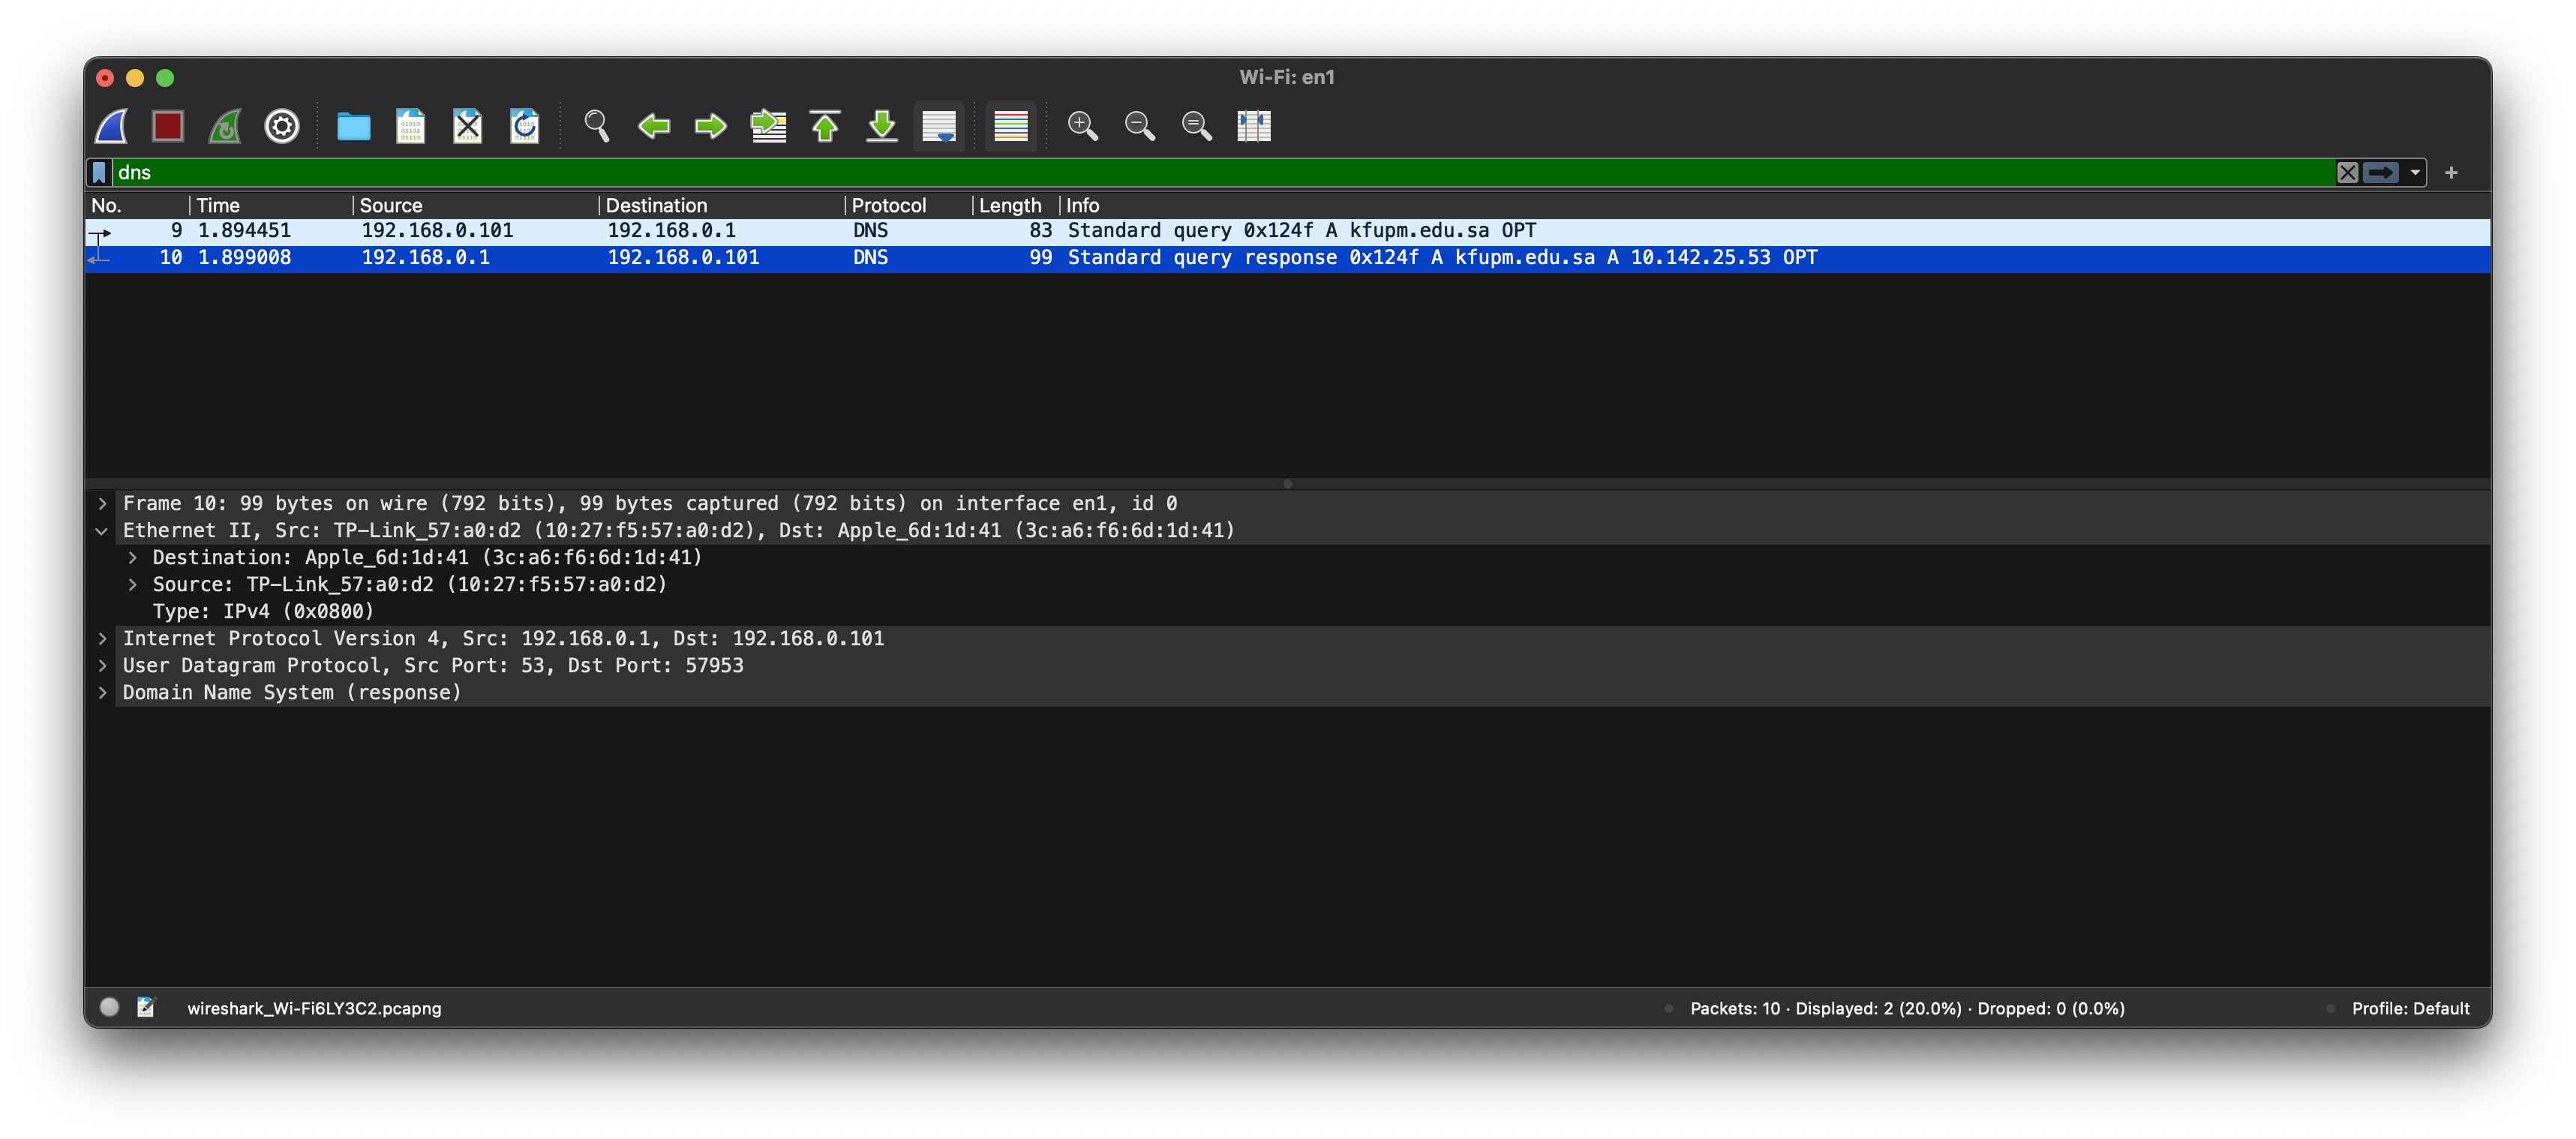
\includegraphics[width=0.8\textwidth]{figures/norm-op.png}
  \caption{I used \c{dig kfupm.edu.sa} as test to see where the packet will travell thru. It passes thru the wireless gateway, no MITM exists.}
	\label{fig:norm-op}
\end{figure}

Also, see Figure~\ref{fig:arp-norm} for the victims's ARP table in normal operation.

\begin{figure}[ht]
	\centering
	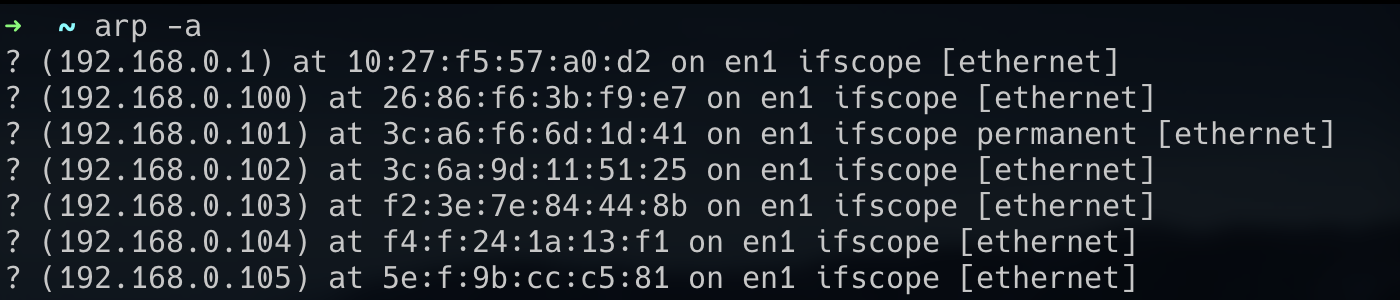
\includegraphics[width=0.8\textwidth]{figures/arp-norm.png}
  \caption{This is the ARP table for victim's machine in normal operation, notice the gateway IP address as well as that for attacker.}
	\label{fig:arp-norm}
\end{figure}


\section{Launching Attack}
\subsection{Get MAC addresses}
To start the attack we need the the corresponding MAC addresses of both the network gateway and victime. I'll use \c{scapy} in interactive mode to send an ARO request to get theier MAC addresses. See Figure~\ref{fig:get-mac} for the commands that I used.

\begin{figure}[ht]
	\centering
	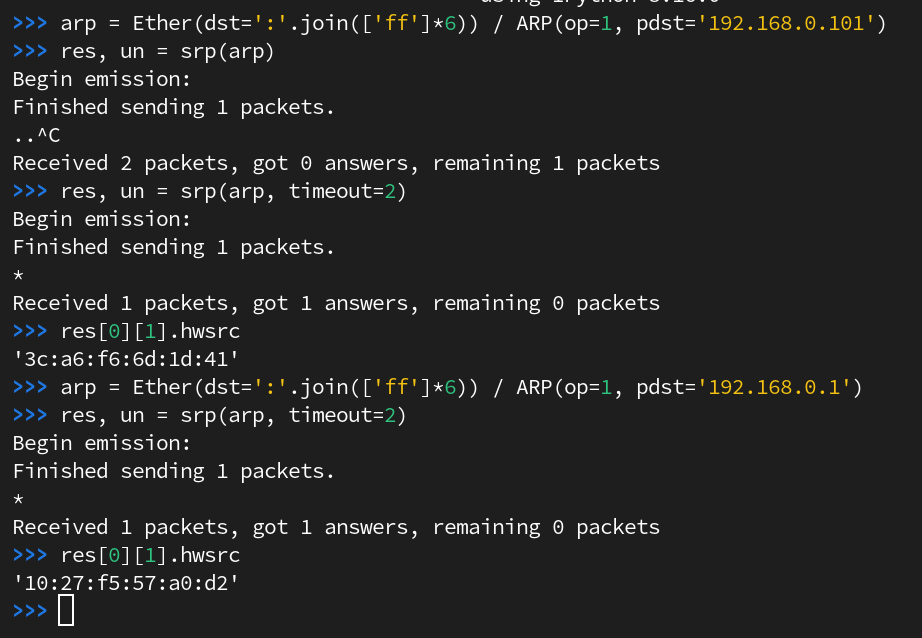
\includegraphics[width=0.8\textwidth]{figures/cmds.png}
  \caption{This is the ARP table for victim's machine in normal operation, notice the gateway IP address as well as that for attacker.}
	\label{fig:get-mac}
\end{figure}

Now for the victim machin: IP address is \c{192.168.0.101} and MAC is \c{3c:a6:f6:6d:1d:41} \\
for the gateway router: IP address is \c{192.168.0.1} and MAC is \c{10:27:f5:57:a0:d2}

\subsection{Spoof ARP Table}

Note: In ARP layer, hwsrc and hwdst represent MAC address of source and destination respectively, while psrc and pdst represent the IP address of source and destination respectively.
Also I run this command to allow port forwarding from the attacker's machine to the corresponding  dst machine: \c{echo 1 > /proc/sys/net/ipv4/ip\_forward}
See the commnads to spoof the victim ARP table Figure~\ref{fig:arp-pois}.

\section{ARP Table}
Let's see the victim's ARP table after attack, in Figure~\ref{fig:arp-pois}.

\begin{figure}[ht]
	\centering
	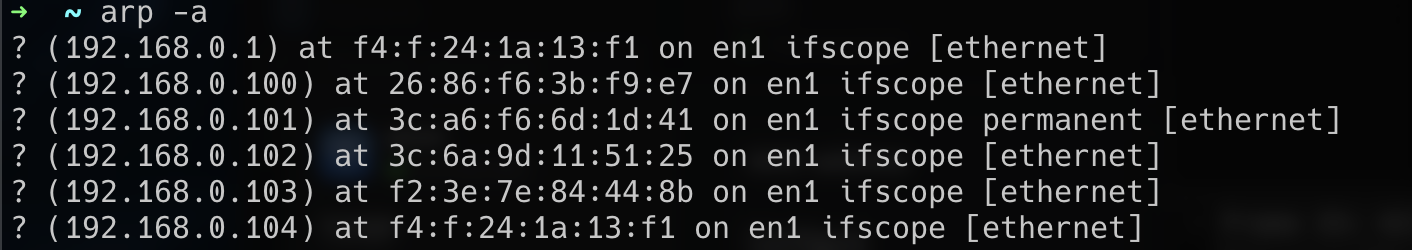
\includegraphics[width=0.8\textwidth]{figures/poisoned-arp.png}
  \caption{We can see now in the victim's ARP table the MAC address is the same is that for the attacker machine with an IP \c{192.168.0.104}.}
	\label{fig:arp-pois}
\end{figure}


\begin{figure}[ht]
	\centering
	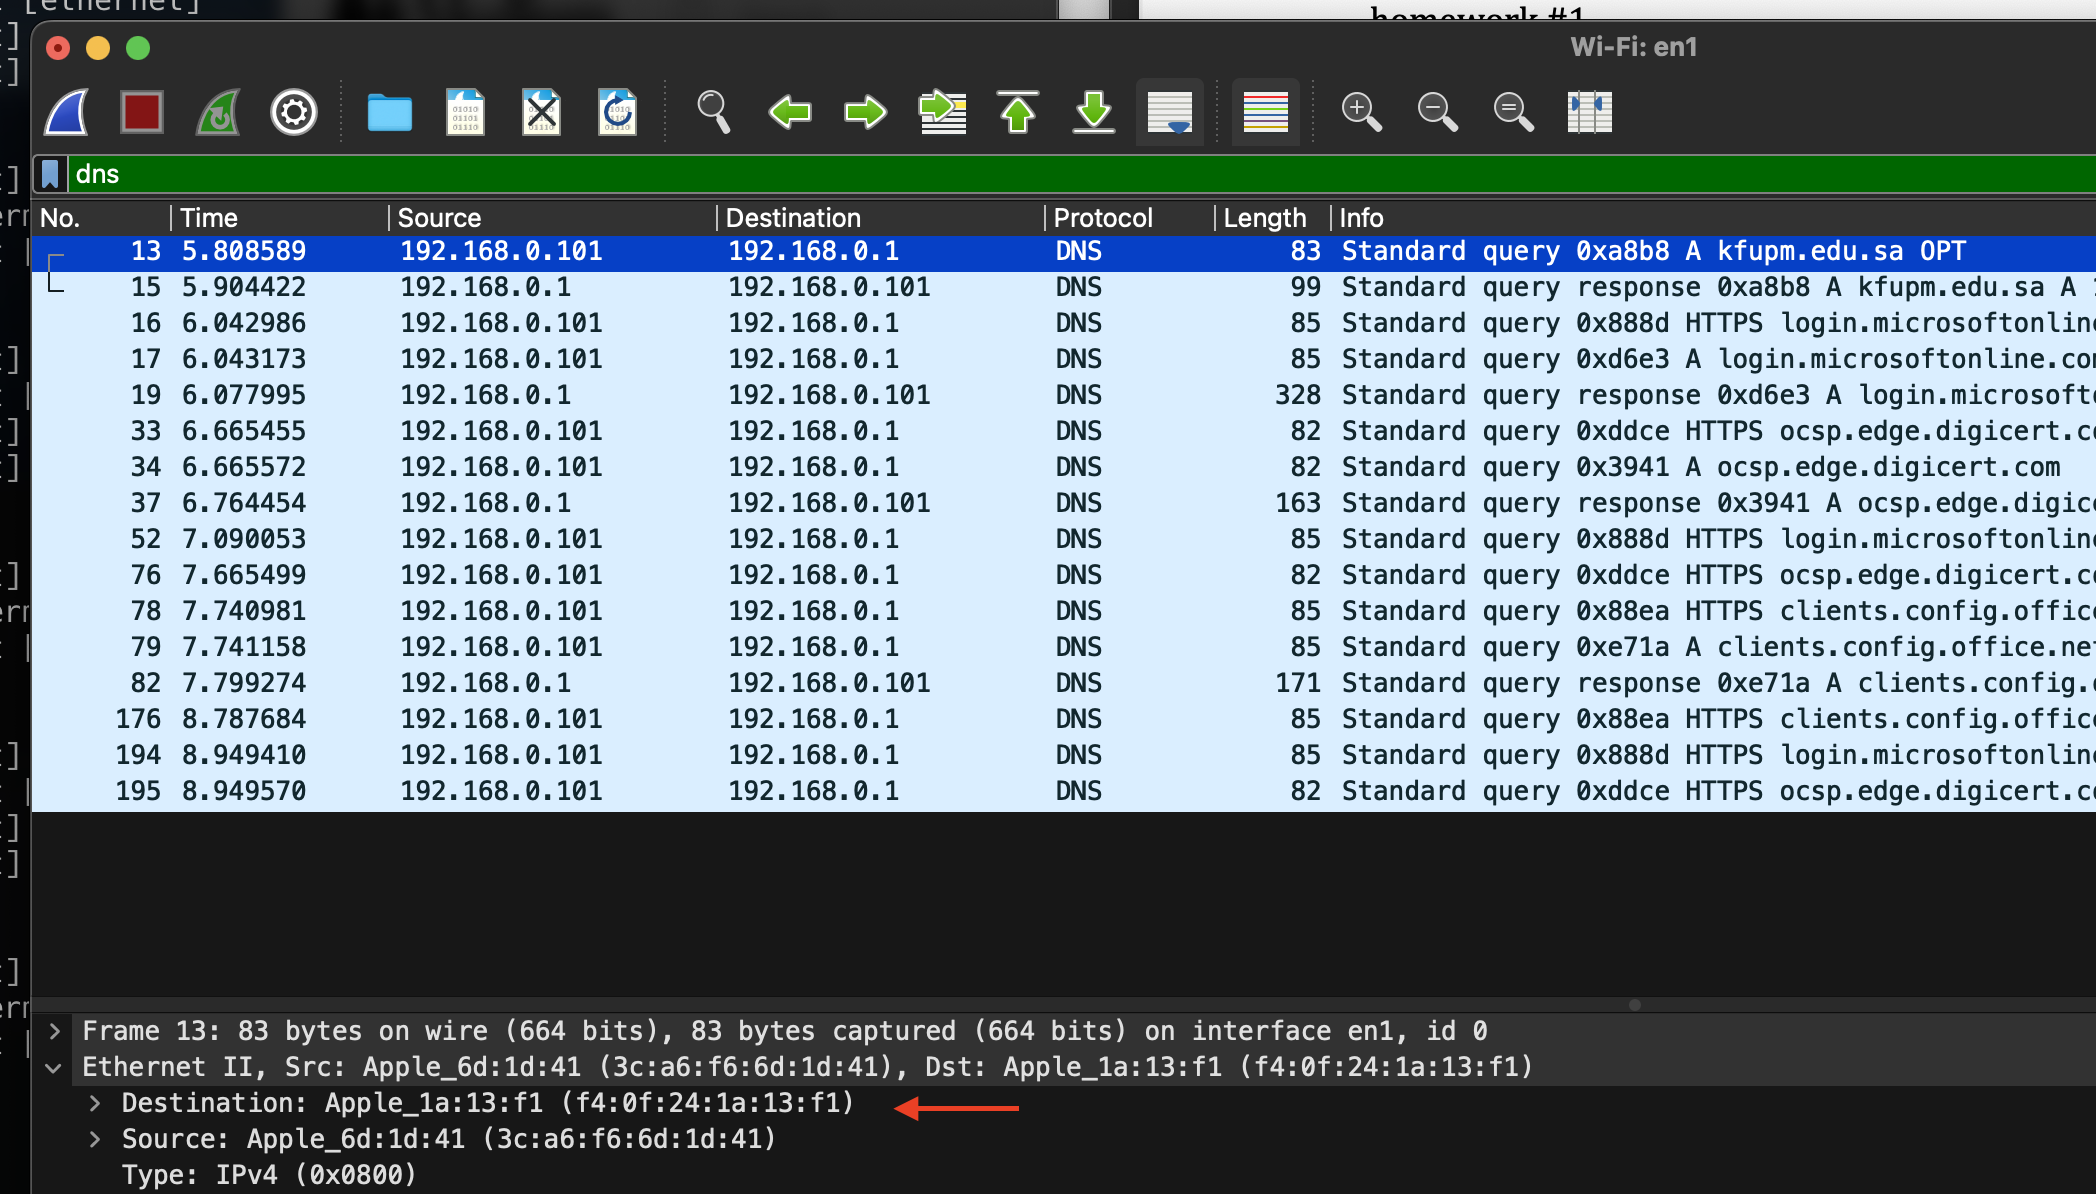
\includegraphics[width=0.8\textwidth]{figures/dns-after.png}
  \caption{We send a dig request form the victim and in wireshark we see indeed the packet goest to the attacker machine first, MITM.}
	\label{fig:get-mac}
\end{figure}

\begin{figure}[ht]
	\centering
	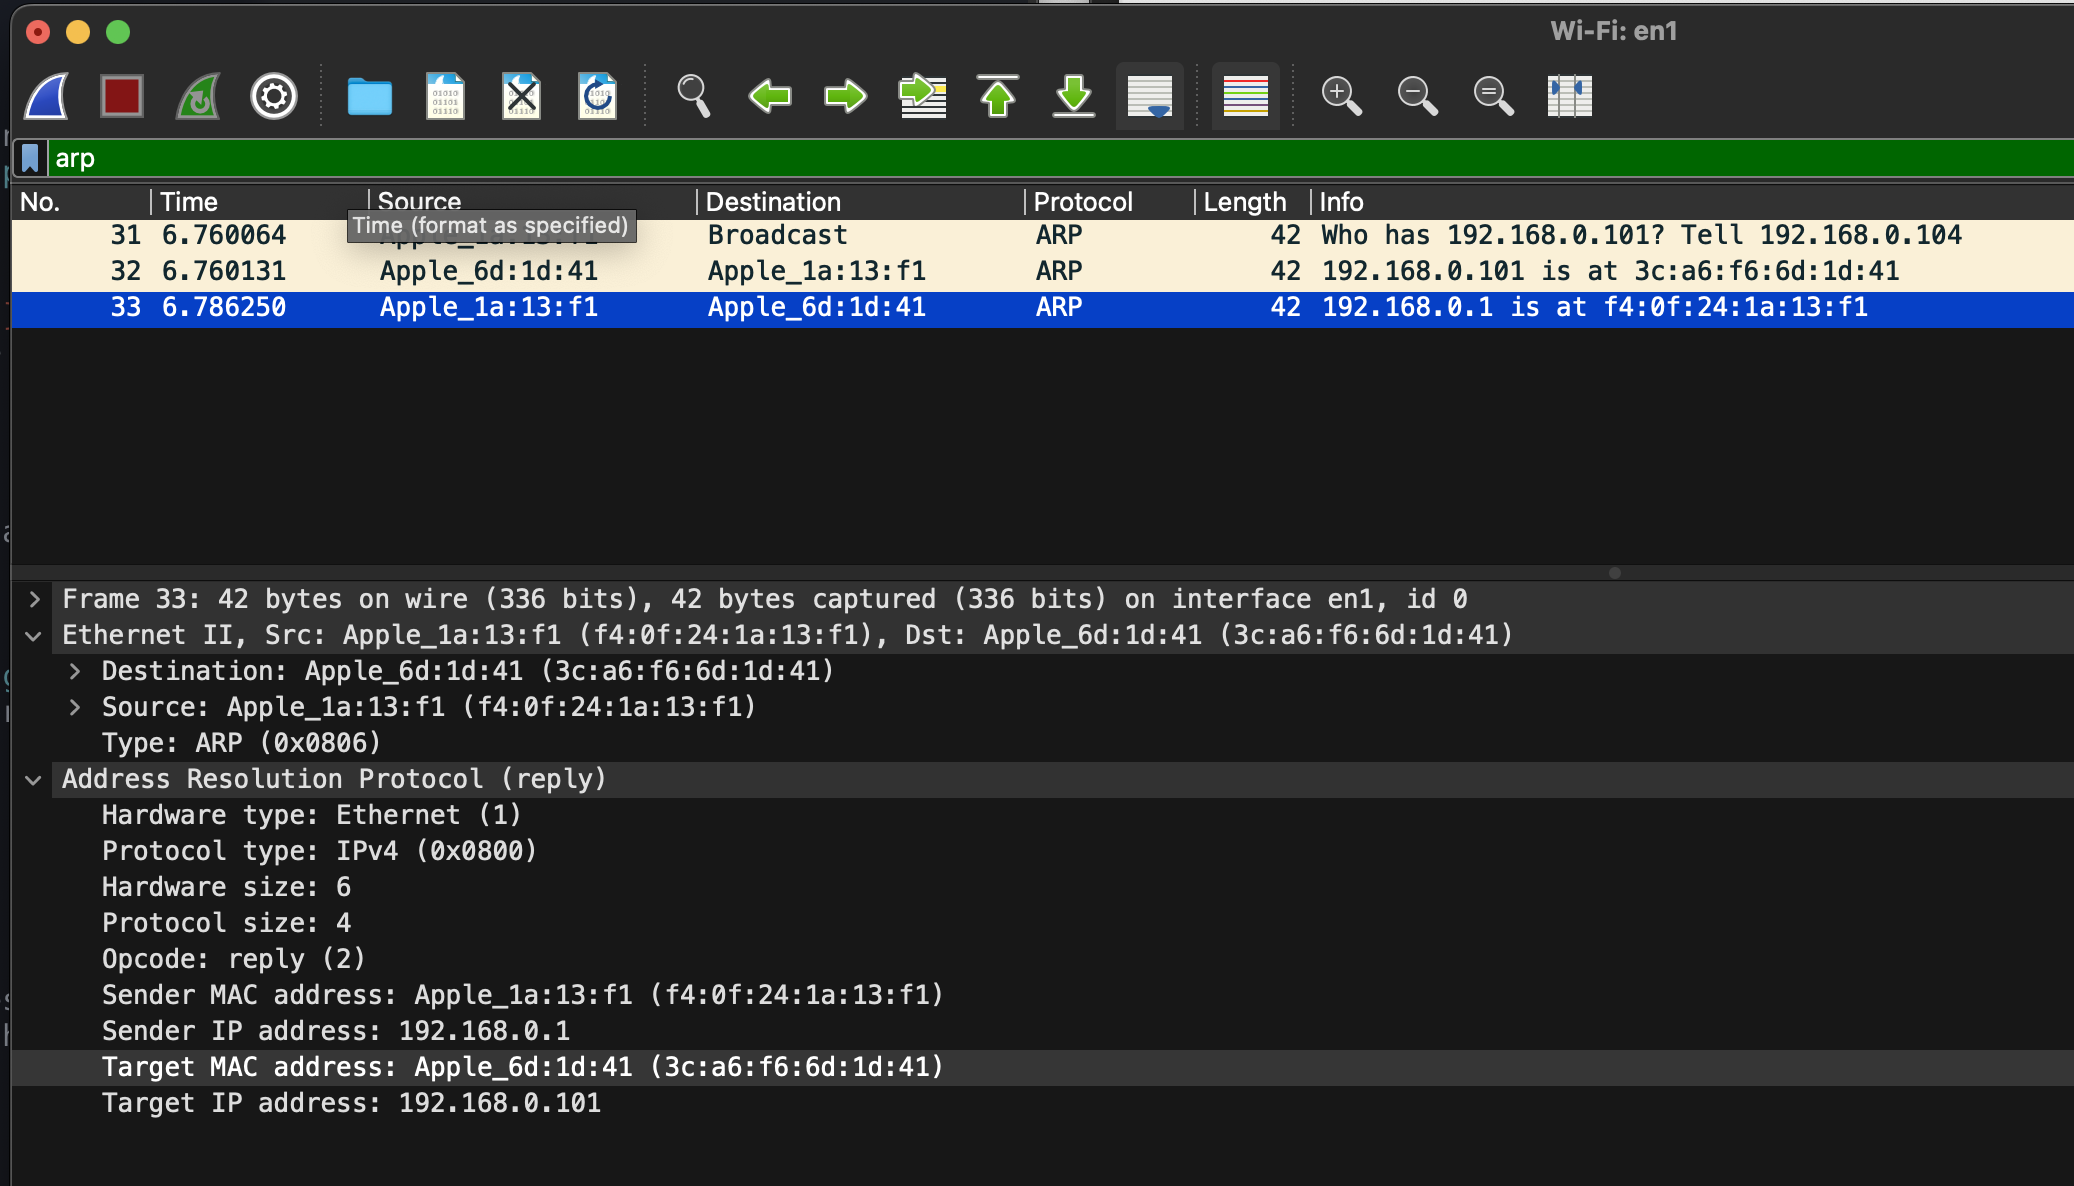
\includegraphics[width=0.8\textwidth]{figures/wire-arp-res.png}
  \caption{This is the ARP table for victim's machine in normal operation, notice the gateway IP address as well as that for attacker.}
	\label{fig:get-mac}
\end{figure}

\begin{figure}[ht]
	\centering
	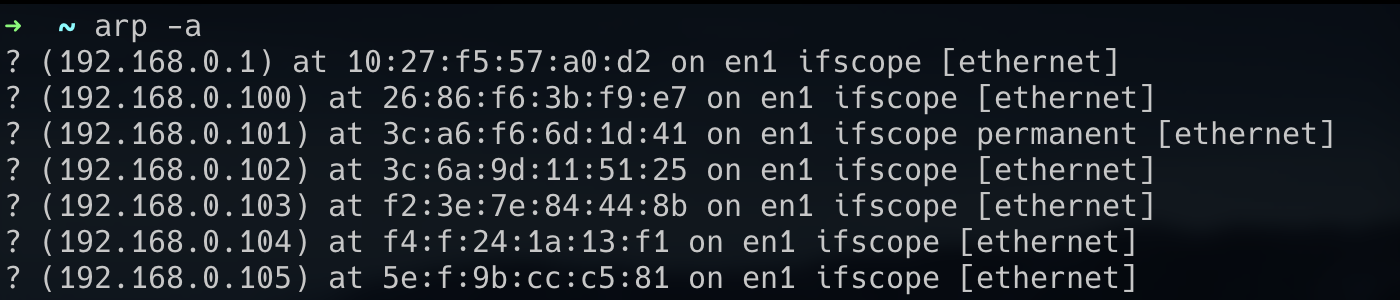
\includegraphics[width=0.8\textwidth]{figures/arp-norm.png}
  \caption{This is the ARP table for victim's machine in normal operation, notice the gateway IP address as well as that for attacker.}
	\label{fig:get-mac}
\end{figure}

\end{document}
